\newcommand{\swaggerlogo}{\vcenteredhbox{
\includegraphics[height=0.07\textheight]{./img/tag_swagger.png}}}
\newcommand{\ramllogo}{\vcenteredhbox{
\includegraphics[height=0.07\textheight]{./img/tag_raml.jpg}}}
\newcommand{\blueprintlogo}{\vcenteredhbox{
\includegraphics[height=0.07\textheight]{./img/tag_apiblueprint.png}}}

\section{Model-First approach}

\subsection{Overview}

\subsubsection{Steps of REST Service Creation}

\begin{frame}[allowframebreaks]
	\frametitle{Steps of REST Service Creation}
	
	Supposing we already defined some \emph{logic architecture} of the system or we `simply' need to wrap some pre-existing SW:
	\setbeamertemplate{enumerate items}[default]
	\begin{enumerate}
		\item Define the mean(s) for user/caller authentication
		\item Identify \emph{resources} and HTTP \emph{verbs} they support
		\item Assign some \emph{route} (URI) to each resource
		\begin{itemize}
			\item Routes can contain one or more \emph{query parameters}
		\end{itemize}
		
		\framebreak
		
		\item For each method supported by each route:
		\begin{enumerate}
			\item Choose one ore more needed authentication means
			\item Define supported request/response \emph{content-types}
			\begin{itemize}
				\item \texttt{application/json}, \texttt{application/xml}, \texttt{text/html}, \ldots			
			\end{itemize}
			\item Define \emph{where} to put \emph{request's arguments}
			\begin{itemize}
				\item Headers, Body, URI, Query	
			\end{itemize}
			\item Define request's arguments \emph{structures}
			\begin{itemize}
				\item \emph{JSON Schema}, \emph{DTD}, \emph{XML Schema}, \ldots
			\end{itemize}
			\item Define \emph{status codes} allowed as \emph{responses} and, for each one:
				\begin{itemize}
					\item \emph{Body}'s structure
					\item \emph{Headers}' structure
				\end{itemize}
		\end{enumerate}
	\end{enumerate}
	
	\framebreak
	
	\begin{exampleblock}{Example: Pet Store - API Routes}
		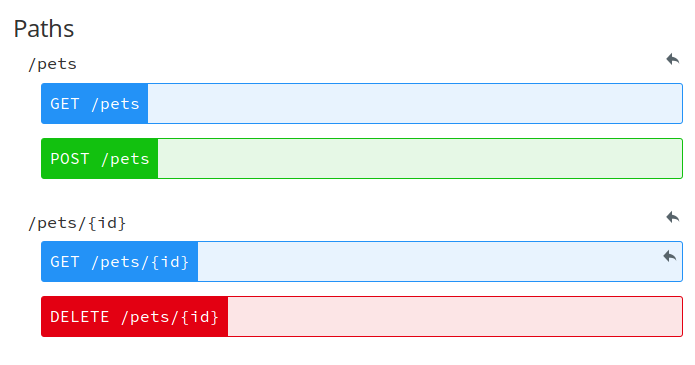
\includegraphics[width=\textwidth]{./img/api_example_paths_alpha.png}
	\end{exampleblock}
	
	\framebreak
		
	\begin{exampleblock}{Example: Pet Store - Route Detail}
		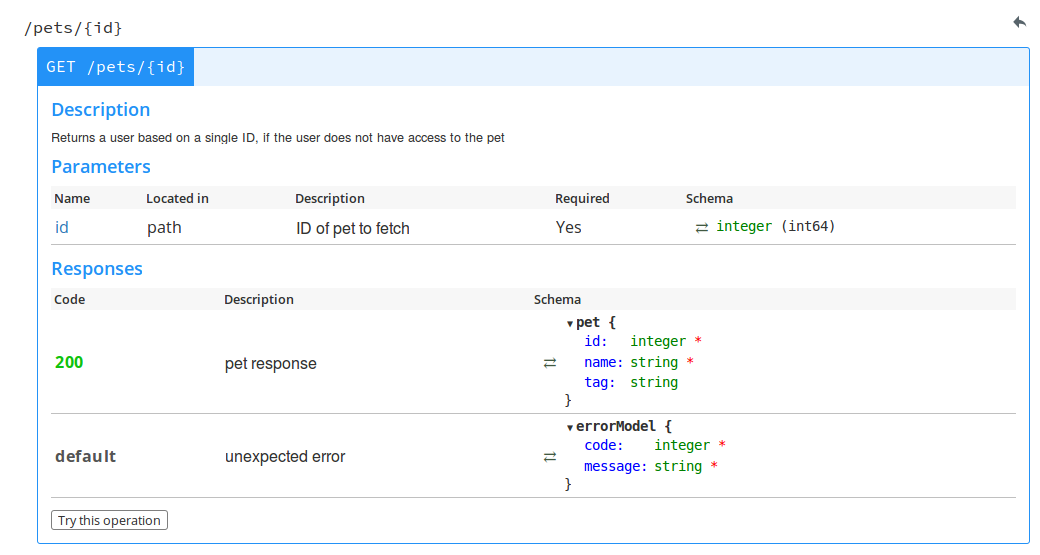
\includegraphics[width=\textwidth]{./img/api_example_route_alpha.png}
	\end{exampleblock}
	
	\framebreak
			
	\begin{exampleblock}{Example: Pet Store - JSON Schemas (Tiping)}
		\begin{tabularx}{\textwidth}{X||X}
			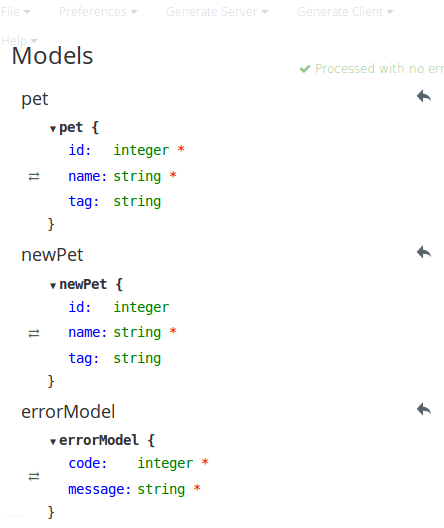
\includegraphics[width=0.48\textwidth]{./img/api_example_schemas1_alpha.png} &
			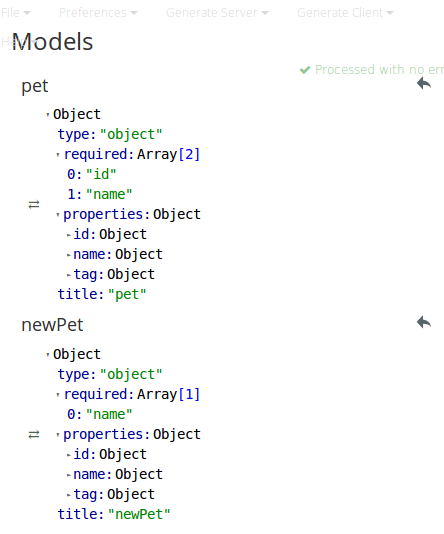
\includegraphics[width=0.48\textwidth]{./img/api_example_schemas2_alpha.png}
		\end{tabularx}
	\end{exampleblock}
	
\end{frame}

\subsubsection{Model-first tools}

\begin{frame} %[allowframebreaks]
	\frametitle{Model-first tools}
	
	What if we had some formal way to model APIs?
	
	\begin{exampleblock}{Swagger}
		 \swaggerlogo\ \url{http://swagger.io}
	\end{exampleblock}
	
	\begin{exampleblock}{RAML - \textbf{R}ESTful \textbf{A}PI \textbf{M}odelling \textbf{L}anguage}	
		\ramllogo\ \url{http://www.raml.org}
	\end{exampleblock}
	
	\begin{exampleblock}{Api Blueprint}
	 	\blueprintlogo\ \url{https://apiblueprint.org/}
	\end{exampleblock}
\end{frame}

\subsection{Swagger}

\subsubsection{Features}

\begin{frame} %[allowframebreaks]
	\frametitle{Swagger features}
	
	\begin{itemize}
		\item[$\checkmark$] JSON/YAML-based modeling language
		\begin{itemize}
			\item[$\times$] a little verbose
		\end{itemize} 
		\item[$\checkmark$] Allows to easily define type schemas
		\item[$\times$] Only explicitly supports Basic authentication, Api Key and OAuth2
		\item[$\checkmark$] Largest and most active developers community
		\item[?] Industry Backing: Reverb, 3Scale, Apigee (NFI)
		\item[$\checkmark$] Largest platform support (Clojure, Go, JS, Java, Node, .Net, PHP, Python, Ruby, Scala)
		\item[$\checkmark$] Web-based editor available at \url{http://editor.swagger.io} or as \texttt{nodejs} module
		\item[$\checkmark$] Generates extremely detailed API which allows for in-app testing
		\begin{itemize}
			\item[$\times$] not-so-easy setup: it's a standalone server
		\end{itemize} 
		\item[$\checkmark$] Lots of tools for editing (\texttt{Swagger Editor}), code generation (\texttt{Swagger Codegen}) or API presentation/navigation (\texttt{Swagger UI})
	\end{itemize}
\end{frame}

\subsubsection{Users example - Swagger}

\begin{frame}[allowframebreaks,fragile]
	\frametitle{Users example - Swagger}
	\begin{exampleblock}{Headers}
		\begin{lstlisting}[language=yaml,basicstyle=\tiny,linewidth=0.48\textwidth] 
			swagger: '2.0'
			info:
			  description: Some description here
			  version: 16.05 acute angle
			  title: Swagger Sample App
			  contact: 
			    name: gciatto
			    email: giovanni.ciatto@gmail.com
			tags:
			  - name: Users
			  - name: Default  
			securityDefinitions:
			  JWT-User:
			    type: apiKey
			    in: header
			    name: Authorization
			    x-jwt-header:
			      alg: HS512
			    x-jwt-payload:
			      iss: localhost
			      aud: localhost
			      role: user
			schemes:
			  - http
		\end{lstlisting}
	\end{exampleblock}
	
	\begin{exampleblock}{JSON Schemas definitions (2 columns)}
		\begin{columns}
		\begin{column}{0.48\textwidth}
		\begin{lstlisting}[language=yaml,basicstyle=\tiny] 
			definitions:
			  Error:
			    type: object
			    required:
			      - message
			      - status
			    properties:
			      message:
			        type: string
			      status:
			        type: integer
			        format: int32
			  Token:
			    type: object
			    required:
			      - token
			    properties:
			      token:
			        type: string
			  User:
			    type: object
			    required:
			      - admin
			      - username
		\end{lstlisting}
		\end{column}
		\begin{column}{0.48\textwidth}	
		\begin{lstlisting}[language=yaml,basicstyle=\tiny] 
			    properties:
			      admin:
			        type: boolean
			        default: false
			      name:
			        type: string
			      surname:
			        type: string
			      username:
			        type: string
			  UserAuth:
			    type: object
			    required:
			      - password
			      - username
			    properties:
			      password:
			        type: string
			      username:
			        type: string
		\end{lstlisting}
		\end{column}
		\end{columns}
	\end{exampleblock}
	
	\begin{exampleblock}{Paths (columns 1-2 / 4)}
		\begin{columns}
		
		\begin{column}{0.48\textwidth}
		\begin{lstlisting}[language=yaml,basicstyle=\tiny]
			paths:
			  /users:
			    get:
			      tags:
			        - Users
			      operationId: getUsers
			      consumes: []
			      produces:
			        - application/json
			      parameters:
			        - name: limit
			          in: query
			          required: false
			          type: integer
			          format: int64
			          x-example: 10
			        - name: offset
			          in: query
			          required: false
			          type: integer
			          format: int64
			          x-example: 0
			      responses:
		\end{lstlisting}
		\end{column}
		
		\begin{column}{0.48\textwidth}
		\begin{lstlisting}[language=yaml,basicstyle=\tiny]
			        '200':
			          description: |
			            The request has succeeded
			          schema:
			            $ref: '#/definitions/User'
			    post:
			      tags:
			        - Users
			      operationId: postUsers
			      consumes: []
			      produces: []
			      parameters: []
			      responses:
			        '200':
			          description: OK
			  '/users/{username}':
			    get:
			      tags:
			        - Users
			      consumes: []
			      produces:
			        - application/json
			      parameters:
		\end{lstlisting}
		\end{column}
		
		\end{columns}
	\end{exampleblock}
	
\begin{exampleblock}{Paths (columns 3-4 / 4)}
		\begin{columns}
		
		\begin{column}{0.48\textwidth}
		\begin{lstlisting}[language=yaml,basicstyle=\tiny]
			        - name: username
			          in: path
			          required: true
			          type: string
			      responses:
			        '200':
			          description: Success
			          schema:
			            $ref: '#/definitions/User'
			        '401':
			          description: Error 401
			          schema:
			            $ref: '#/definitions/Error'
			        '404':
			          description: Error 404
			          schema:
			            $ref: '#/definitions/Error'
			      security: 
			        - JWT-User: []
			  '/users/{username}/token':
			    post:
			      tags:
			        - Users
		\end{lstlisting}
		\end{column}
		
		\begin{column}{0.48\textwidth}
		\begin{lstlisting}[language=yaml,basicstyle=\tiny]
			      consumes:
			        - application/json
			      produces:
			        - application/json
			      parameters:
			        - name: username
			          in: path
			          required: true
			          type: string
			        - in: body
			          name: body
			          required: false
			          schema:
			            $ref: '#/definitions/UserAuth'
			      responses:
			        '200':
			          description: Success
			          schema:
			            $ref: '#/definitions/Token'
			        '401':
			          description: Error 401
			          schema:
			            $ref: '#/definitions/Error'
		\end{lstlisting}
		\end{column}
		
		\end{columns}
	\end{exampleblock}

\end{frame}